% Preamble
% Compile with XeLateX

\documentclass[11 pt,oneside,a4paper,titlepage]{article}
\usepackage{preamble}
\graphicspath{{PIC/}}
%%%%%%%%%%%%%%%%%%%%%%%%%%%%%%%%%%%%%%%%%%%%%%%%%%%%%%%%%%%%%%%%%%%%%%%%%%%%%%%%%%%%%%
\begin{document}

\sidebar{sideBarColor!25}
\simpleheader{titleBackColor}{Jack}{Sparrow}{Captain | Pirate}{white}

% Start Minipages
\vspace*{3.49cm}% start 8 cm from the top of the page}
    \adjustbox{valign=t}{\begin{minipage}{7.3cm} % large 7.4 cm from the top
    \vspace*{1.2cm} % text starts 1cm under the top of the minipage

        % Picture
        \begin{center}
        \begin{tikzpicture}
            \node[
            circle,
            minimum size=\cvPictureWidth,
            path picture={
            \node at (path picture bounding box.center){
             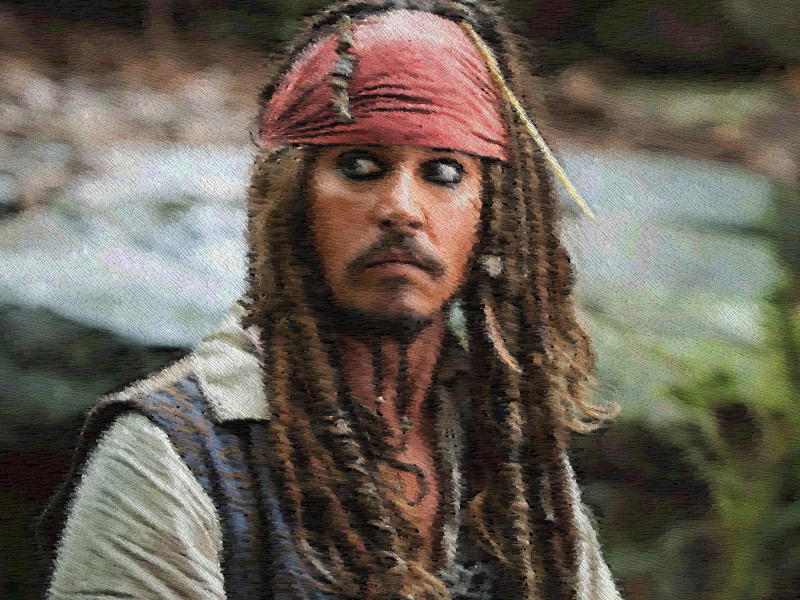
\includegraphics[width=\cvPictureWidth]{Picture.jpg}
             };
             }]
            {};
        \end{tikzpicture}
        \end{center}

        %%%%%%%%%%%%%%%%%%%%%%%%%%%%%%%%%%%%%%%%%%%%%%%%%%%%
        % Profile section
        \ruleline{\textbf{About me}}
        Gabriel %

        %%%%%%%%%%%%%%%%%%%%%%%%%%%%%%%%%%%%%%%%%%%%%%%%%%%
        % Contact Section
        \ruleline{\textbf{Contact}}
        \begin{tikzpicture}[every node/.style={inner sep=0pt, outer sep=0pt}]
        \matrix [
        column 1/.style={anchor=center,contactIcon},
        column 2/.style={anchor=west,align=left,contactIcon},
        column sep=5pt,
        row sep=5pt] (contact) {
        \node{\faMale};
         & \node{Born on xx/xx/1690, Age ??};\\
        \node{\faEnvelope};
         & \node{\href{mailto:jacksparrow@yahoo.it}{jacksparrow@yahoo.it}};\\
         \node{\faEnvelopeO};
         & \node{\href{mailto:jacksparrow2@yahoo.it}{jacksparrow2@yahoo.it}};\\
        \node{\faPhone};
         & \node{+39 xxxxxxxxxx};\\
        \node{\faMapMarker};
        & \node{Tortuga Street 9 \\ ZIPCODE City (TG), Country};\\
        \node{\faLinkedinSquare};
        & \node{\href{your LinkedIn Link here}{jack-sparrow}};\\
        \node{\aiResearchGateSquare};
        & \node{\href{your Research Gate Link here}{Research Gate: Jack}};\\
        \node{\aiOrcid};
        & \node{\href{your Orcid Link here}{ORCID: xxxx-xxxx-xxxx-xxxx}};\\
        \node{\faCar};
        & \node{Car Available, Driving License B};\\
         };
        \end{tikzpicture}

        %%%%%%%%%%%%%%%%%%%%%%%%%%%%%%%%%%%%%%%%%%%%%%%%%%%
        \ruleline{\textbf{Languages}}
        \begin{tikzpicture}[every node/.style={inner sep=0pt, outer sep=0pt}]
        \matrix [
        column 1/.style={anchor=center,contactIcon},
        column 2/.style={anchor=west,align=left,contactIcon},
        column sep=5pt,
        row sep=5pt] (contact) {
        \node{\flag{England.png}};
        & \node{English - Native Language};\\
        \node{\flag{Italy.png}};
        & \node{Italian - Professional Knowledge};\\
        \node{\flag{Spain.png}};
        & \node{Spanish - Basic Knowledge};\\
        \node{\flag{France.png}};
        & \node{French - Professional Knowledge};\\
        };
        \end{tikzpicture}

        %%%%%%%%%%%%%%%%%%%%%%%%%%%%%%%%%%%%%%%%%%%%%%%%%%%%%
        % QR Code
        \begin{center}
            
\includegraphics[width=3.5cm]{QR_Info.png}
        \end{center}

    \end{minipage}} %
    \hfill
%%%%%%%%%%%%%%%%%%%%%%%%%%%%%%%%%%%%%%%%%%%%%%%%%%%%%%%%%
%%%%% MAIN SECTION %%%%%%%%%%%%%%%%%%%%
    \adjustbox{valign=t}{\begin{minipage}{11.3cm}
        \vspace*{1cm}
        \section*{{\faGraduationCap} EDUCATION}

        \MySection{2018-Ongoing}{Ship.png}{Master Degree}{Pirate University}{Tortuga, Caribbean}{Faculty}{A description of your piracy. \\\textbf{Degree: 110/110 cum laude}}

        \vspace*{0.22cm}

        \MySection{2016-2018}{Jolly-Roger.png}{Bachelor Degree}{Tortuga Academy}{East Indies}{Buccaneer}{Attacking and robbing ships at sea. \lipsum[150]\\\textbf{Degree: 110/110}}

        %%%%%%%%%%%%%%%%%%%%%%%%%%%%%%%%%%%%%%%%%%%%%%%%%%%
        % Work Experience
        \section*{{\faSuitcase} WORK EXPERIENCE}

        \MySectionNoPic{2018-Today}{Captain of the Black Pearl}{Tortuga, Caribbean}{Your Company}{Found a secret treasure, lost the ship. \lipsum[12]}

        \vspace*{0.22cm}

        \MySectionNoPic{2010-2020}{Freelance Pirate}{Tortuga, Caribbean}{Buccaneering SPA}{\lipsum[24]}

        %%%%%%%%%%%%%%%%%%%%%%%%%%%%%%%%%%%%%%%%%%%%%%%%%%%
        % Publications
        \section*{{\aiOBP} PUBLICATIONS}

        \publication{Journal Article}{1729}{How I almost got killed by Lady Swan}{Jack Sparrow, Elizabeth Swan, William Turner III, Davy Jones}{Tortuga Printing Press}{10.3389/doicodedoicode}

        \vspace*{0.22cm}

        \publication{Abstract}{1725}{The Kraken and other stories}{Jack Sparrow, Hector Barbossa, Jack the Monkey, Joshamee Gibbs}{1st Congress of Pirate}{10.1016/doicodedoicode}

        \vspace*{0.22cm}

        \publication{Conference Proceedings}{1724}{How I lost my ship and how to get it back}{Jack Sparrow}{Conference in Tortuga}{10.5220/doidoidoi}

        \vspace*{0.22cm}

    \end{minipage}} %

%%%%%%%%%%%%%%%%%%%%%%%%%%%%%%%%%%%%%%%%%%%%%%%%%%%%%%%%%%%%
% Second Page
\newpage

\sidebar{sideBarColor!25}
\newpageheader{titleBackColor}{Jack}{Sparrow}{Pirate \faLightbulbO \hspace{1mm} Captain}{white}

% %%%%%%%%%%%%%%%%%%%%%%%%%%%%%%%%%% SIDEBAR %%%%%%%%%%%%%%%%%%%
\adjustbox{valign=t}{%
\begin{minipage}{7.3cm}
\vspace*{0.4cm} % text starts 0.4cm under the top the header

    %%%%%%%%%%%%%%%%%%%%%%%%%%%%%%%%%%%%%%%%%%%%%%%%%%%%
    % Skill and Strengths
    \ruleline{\textbf{Soft Skills and Strengths}}
    \vspace*{-0.5cm}
    \begin{center}
        \cvtag{Creativity}\cvtag{Curiosity}\cvtag{Flexibility}\cvtag{Self Confidence}\cvtag{Ability to Plan and Organize} \cvtag{Autonomy}\cvtag{Adaptability} \cvtag{Eye for Details}\cvtag{Problem Solving}\cvtag{Team Working}\cvtag{Love Learning New Things}\cvtag{Leadership}\cvtag{Good Communication}\cvtag{Managing Information}\cvtag{Diplomacy}\cvtag{Good Listener}\cvtag{Patience}
    \end{center}

    %%%%%%%%%%%%%%%%%%%%%%%%%%%%%%%%%%%%%%%%%%%%%%%%%%%%
    % Professional Skills
    \ruleline{\textbf{Professional Skills}}
    \begin{center}
        \cvtag{Skill 1}\cvtag{Skill 2}\cvtag{Skill 3}\cvtag{Skill 4}\cvtag{Skill 5}
    \end{center}

    %%%%%%%%%%%%%%%%%%%%%%%%%%%%%%%%%%%%%%%%%%%%%%%%%%%
    % Other Interests
    \ruleline{\textbf{Other Interests}}
    \small
    \begin{multicols}{2}
        \begin{itemize}
            \item  Guitar \flag{Guitar.png}
            \item  Piano \flag{Piano.png}
            \item  Chess \flag{Chess.png}
            \item  Gym \flag{Gym.png}
            \item  Travels \flag{Travels.png}
            \item  Movies \flag{movie2.png}
            \item  Books \flag{Books.png}
    \end{itemize}
    \end{multicols}

     %%%%%%%%%%%%%%%%%%%%%%%%%%%%%%%%%%%%%%%%%%%%%%%%%%%%%
        % QR Code
        \ruleline{\textbf{Download My CV}}
        \scriptsize
        \centering
        Download my CV via the QR below \aiOverleaf.
        \begin{center}
            \quad
            \qrcode[height=2cm]{
                https://www.dropbox.com/sh/k5pheguf9jrur8x/AADpyjYJi7V5bhPyJeP3H74ea?dl=0} \\
            \vspace*{0.5cm}
        \end{center}

\end{minipage}
}%
\hfill
%%%%%%%%%%%%%%%%%%%%%%%%%%%%%%%%%%% MAIN %%%%%%%%%%%%%%%%%%%%%%%%%
\adjustbox{valign=t}{%
\begin{minipage}{11.3cm}
    \vspace*{0.4cm}
    %%%%%%%%%%%%%%%%%%%%%%%%%%%%%%%%%%%%%%%%%%%%%%%%%%%
    % Peer Reviews
    \section*{{\faBook} ACADEMIC PEER REVIEWS}
    \footnotesize I did academic peer review for the following journals:
    \begin{itemize}
        \footnotesize
         \item{\textbf{Scientific Piracy}, IF: 4.996 (1720), September 1720;}
     \end{itemize}

    %%%%%%%%%%%%%%%%%%%%%%%%%%%%%%%%%%%%%%%%%%%%%%%%%%%
    % Information Technology Skills
    \section*{{\faDesktop} INFORMATION TECHNOLOGY SKILLS}

    \ITCcompetence{Data Analysis}{
    \textbf{MATLAB}: \textit{Higly Specialized}\\
    \textbf{Wolfram Mathematica}: \textit{Intermediate}\\
    \textbf{Jupiter Notebook}: \textit{Intermediate}\\
    }

    \vspace*{0.22cm}

    \ITCcompetence{Modeling and Simulation}{
    \textbf{Simulink} : \textit{Intermediate}  \\
    \textbf{LTSpice}: \textit{Intermediate}
    }

    \vspace*{0.22cm}

    \ITCcompetence{Audio Processing}{
    \textbf{Reaper} : \textit{Advanced}  \\
    }

    \vspace*{0.22cm}

    \ITCcompetence{Office Automation}{
    \textbf{MS Office (Excel, Word, PowerPoint)}: \textit{Higly Specialized}\\
    \textbf{\LaTeX}: \textit{Advanced}\\
    }

    %%%%%%%%%%%%%%%%%%%%%%%%%%%%%%%%%%%%%%%%%%%%%%%%%%%
    % Programming Languages
    \section*{{\faCode} PROGRAMMING LANGUAGES}
    \vspace*{-0.5cm}
    \begin{multicols}{2}
    \begin{itemize}
    \footnotesize
        \item \textbf{Matlab}: Highly Specialised
        \item \textbf{Python}: Advanced
        \item \textbf{SQL}: Intermediate
        \item \textbf{C/C++}: Intermediate
        \item \textbf{Java}: Basic
        \item[\vspace{\fill}]
    \end{itemize}
    \end{multicols}

    %%%%%%%%%%%%%%%%%%%%%%%%%%%%%%%%%%%%%%%%%%%%%%%%%%%
    % Certificates
    \section*{{\faCertificate} CERTIFICATES}

    \adjustbox{valign=t}{\begin{minipage}{2cm}
    \begin{center}
        
\includegraphics[width=1.2cm]{IBM.png}
    \end{center}
    \end{minipage}}
    \hfill \vline \hfill
    \adjustbox{valign=t}{\begin{minipage}{9cm}
        \begin{itemize}
            \scriptsize
            \item Python for Data Science, AI \& Development (\textit{Coursera, 2022})
        \end{itemize}
    \end{minipage}}

    \vspace*{0.2cm}

    \adjustbox{valign=t}{\begin{minipage}{2cm}
    \begin{center}
        
\includegraphics[width=2cm]{Matlab.png}
    \end{center}
    \end{minipage}}
    \hfill \vline \hfill
    \adjustbox{valign=t}{\begin{minipage}{9cm}
        \begin{itemize}
            \scriptsize
            \item Pirate Processing with MATLAB (\textit{Mathworks, 2022})
            \item Signal Processing with MATLAB (\textit{Mathworks, 2022})
            \item Deep Learning with MATLAB (\textit{Mathworks, 2022})
            \item Machine Learning with MATLAB (\textit{Mathworks, 2021})
        \end{itemize}
    \end{minipage}}

    \vspace*{0.2cm}

    \adjustbox{valign=t}{\begin{minipage}{2cm}
    \begin{center}
        
\includegraphics[width=1.2cm]{google.png}
    \end{center}
    \end{minipage}}
    \hfill \vline \hfill
    \adjustbox{valign=t}{\begin{minipage}{9cm}
        \begin{itemize}
            \scriptsize
            \item How to became a Web Pirate (\textit{Google Pirate School, 2022})
            \item item 2
            \item item 3
            \item item 4
        \end{itemize}
    \end{minipage}}

    \vspace*{0.2cm}

\end{minipage}}


\end{document}
